\bivtask{Radiosity mit Povray}{2}
%
Im Verzeichnis \bivfolder{/home/bildgen/Aufgaben/povray-3} finden Sie die 
Datei \texttt{radiosity.pov}. Erweitern Sie 
das Povray-Skript an den markierten Stellen. Aktivieren Sie die 
Radiosity-Implementierung Povrays durch Setzen von „useRadiosity“. Sie 
sollten nun farbige Gegenstände so platzieren, dass Sie auf dem weißen 
Quader ein „Abfärben“ erkennen können. Das folgende Bild zeigt ein
Beispiel für die Platzierung der Objekte, in dem allerdings Radiosity 
noch nicht aktiviert ist:
\begin{center}
  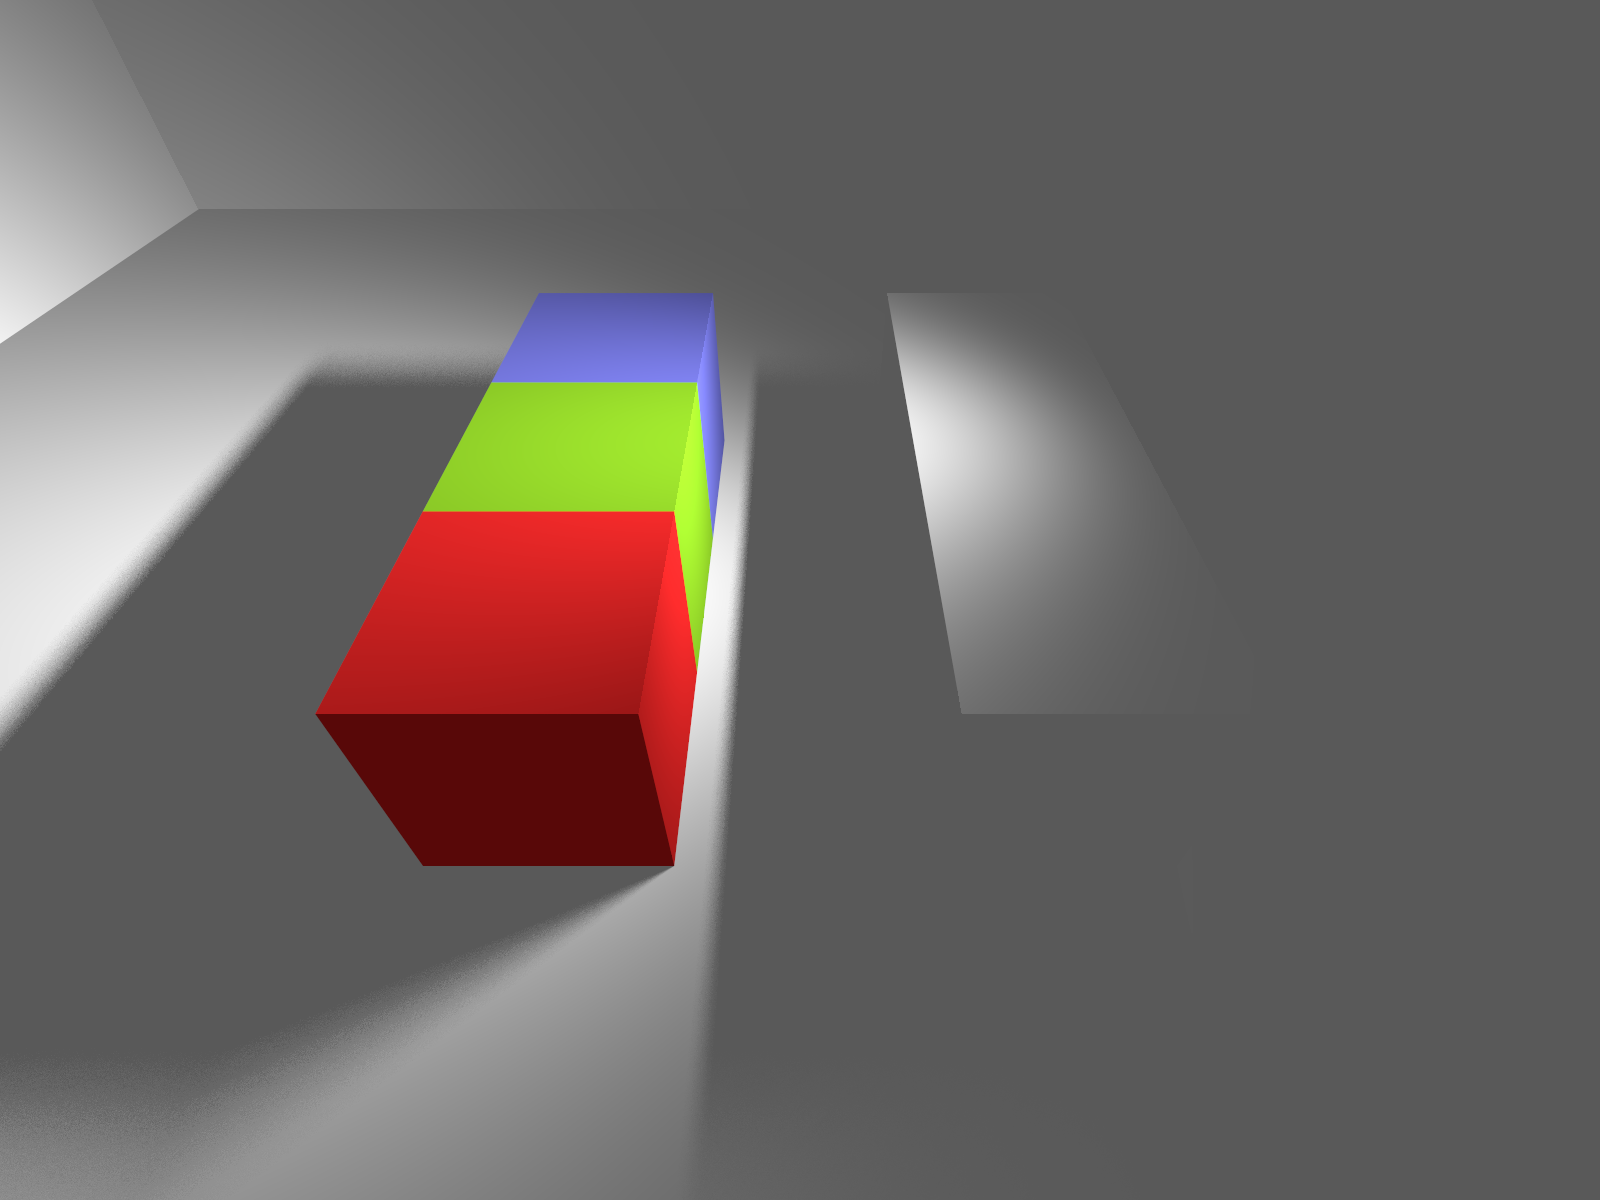
\includegraphics[width=0.5\textwidth]{radiosity.png}
\end{center}
